
\documentclass[11pt,letterpaper]{article}

% Load some basic packages that are useful to have
% and that should be part of any LaTeX installation.
%
% be able to include figures
\usepackage{graphicx}
% get nice colors
\usepackage{xcolor}

% change default font to Palatino (looks nicer!)
\usepackage[latin1]{inputenc}
\usepackage{mathpazo}
\usepackage[T1]{fontenc}
% load some useful math symbols/fonts
\usepackage{latexsym,amsfonts,amsmath,amssymb}

% comfort package to easily set margins
\usepackage[top=1in, bottom=1in, left=1in, right=1in]{geometry}

% control some spacings
%
% spacing after a paragraph
\setlength{\parskip}{.15cm}
% indentation at the top of a new paragraph
\setlength{\parindent}{0.0cm}


\begin{document}

\begin{center}
\Large
Ay190 -- Worksheet 14\\
Anthony Alvarez\\
Date: February 27, 2014
\end{center}

\section{SPH Shock}

We implement a 1D SPH Code for a Shock Tube with the following parameters on a 
domain of $[-0.5,0.5]$ with
$r= 0$, $\rho_L = 1.0$, $\epsilon_L = 2.5$, $v_L = 0$, and on the right side
$\rho_R = 0.25$, $\epsilon_R = 1.795$, $v_R= 0$ and the adiabatic exponent of 
$\gamma = 1.4$ 

\subsection{Shock Develops}

We implement the code in python and run it to a final time of $0.2$. 

We can see in figures ~\ref{fig:0} that the initial density in the left and 
right region are different densities and have a discontinuity. 

\begin{figure}[bth]
\centering
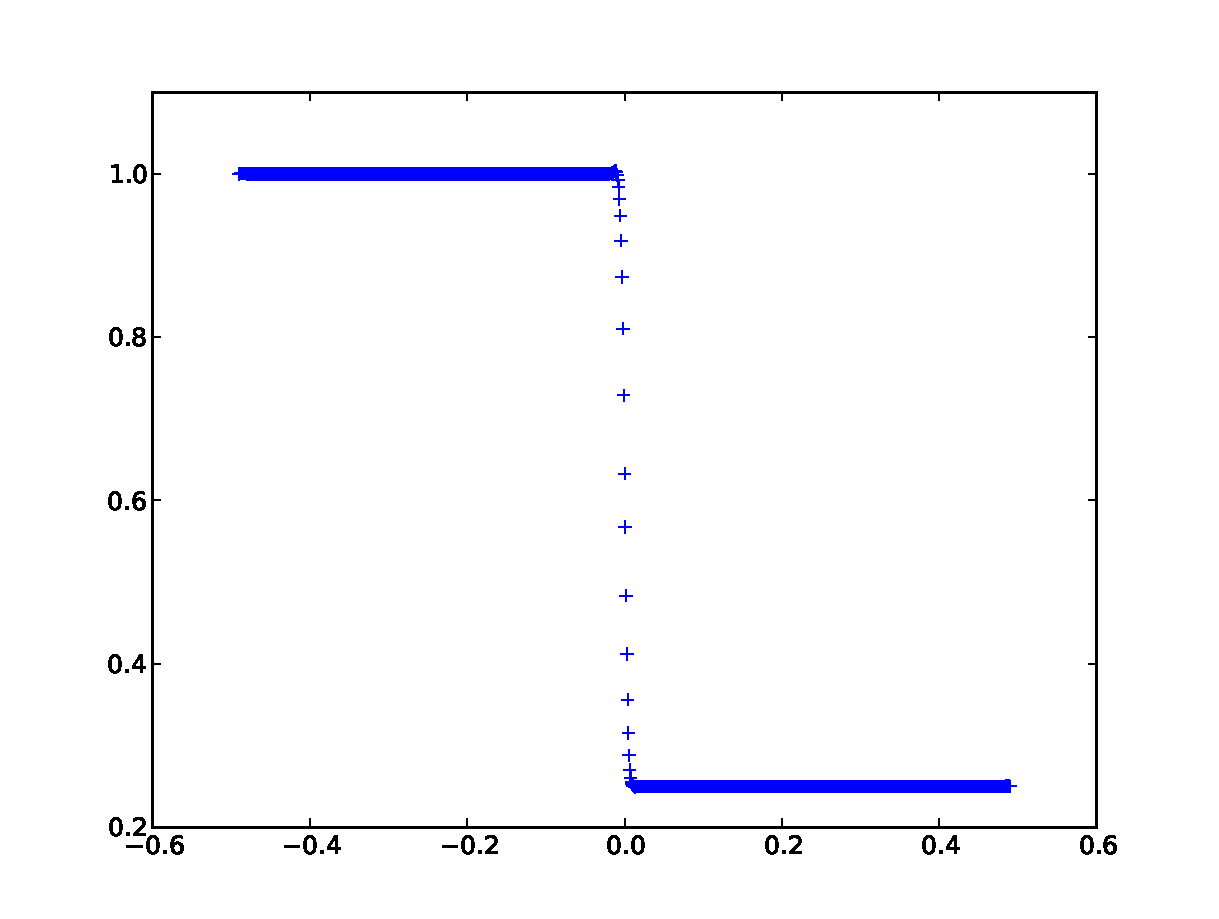
\includegraphics[width=0.5\textwidth]{0.pdf}
\caption{Graph of density with respect to space on the domain 
$[-0.5,0.5]$. At time $t = 0$.}
\label{fig:0}
\end{figure}

\subsubsection{Plateau Devleops}

As it evolves in time we can see the constant density plataus 
develope over time. See figures ~\ref{fig:5}, ~\ref{fig:10}.

\begin{figure}[bth]
\centering
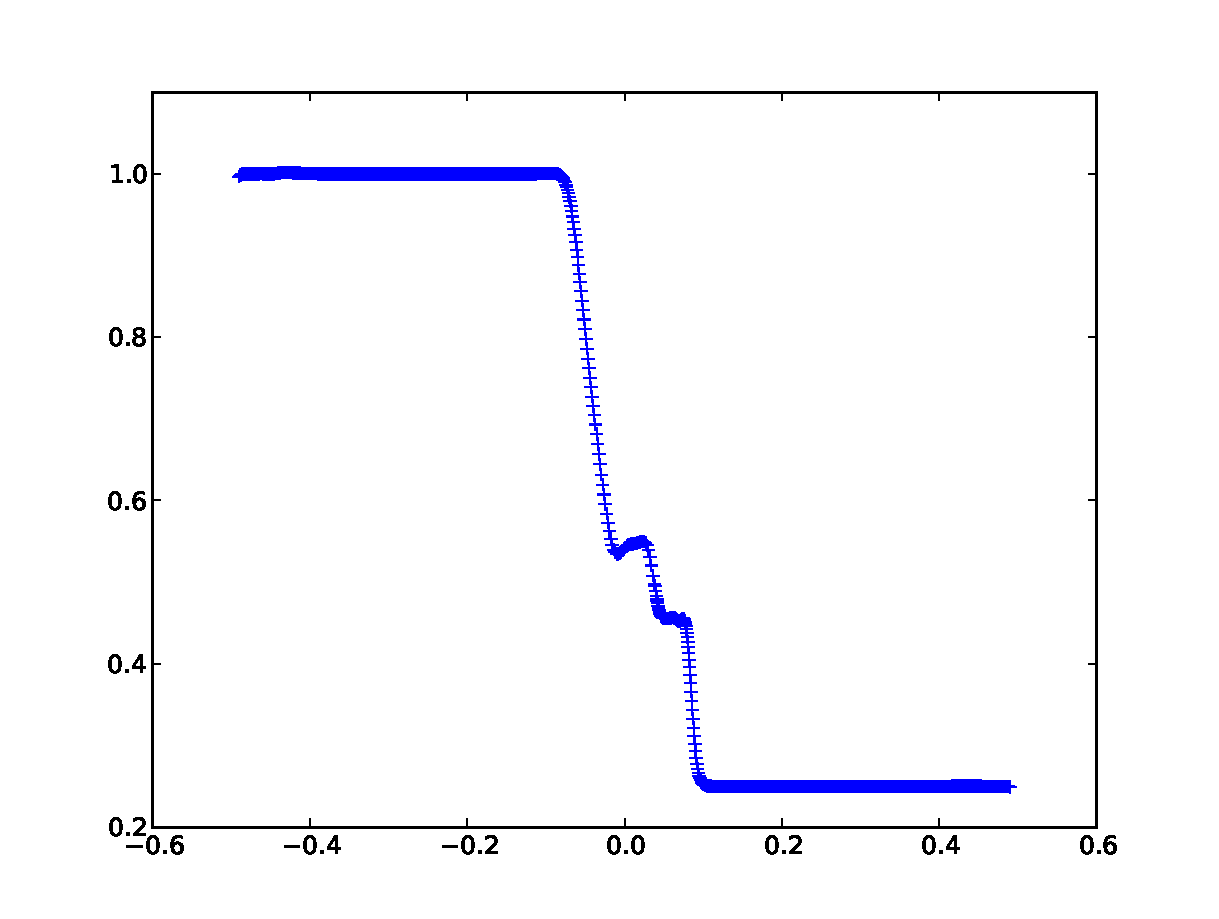
\includegraphics[width=0.5\textwidth]{5.pdf}
\caption{Graph of density with respect to space on the domain 
$[-0.5,0.5]$. At time $t = 0.05$.}
\label{fig:5}
\end{figure}


\begin{figure}[bth]
\centering
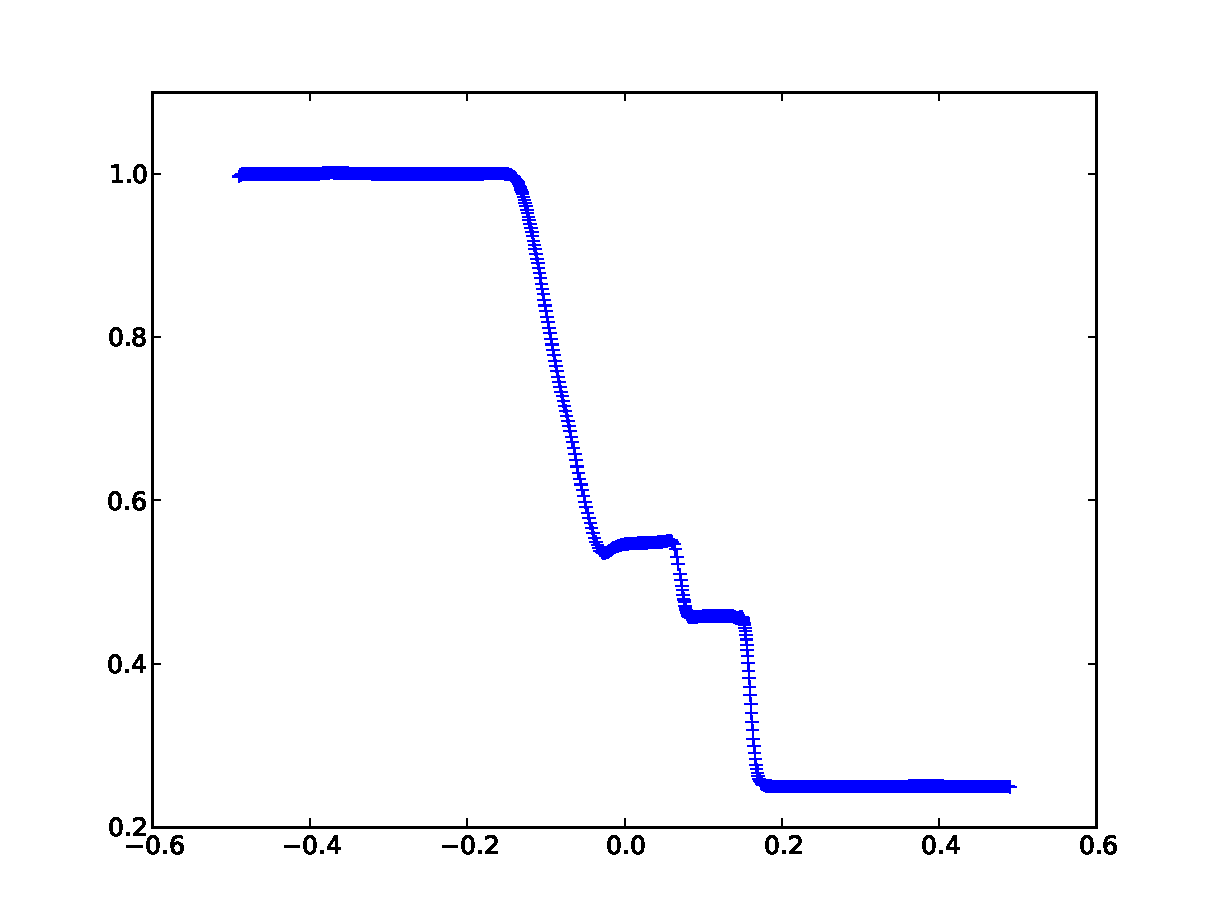
\includegraphics[width=0.5\textwidth]{10.pdf}
\caption{Graph of density with respect to space on the domain 
$[-0.5,0.5]$. At time $t = 0.1$.}
\label{fig:10}
\end{figure}

\subsubsection{Rarefraction Develops}

As time progresses further we can see the rarefraction is more visible in
 ~\ref{fig:15} and at the final time  ~\ref{fig:200}. 

\begin{figure}[bth]
\centering
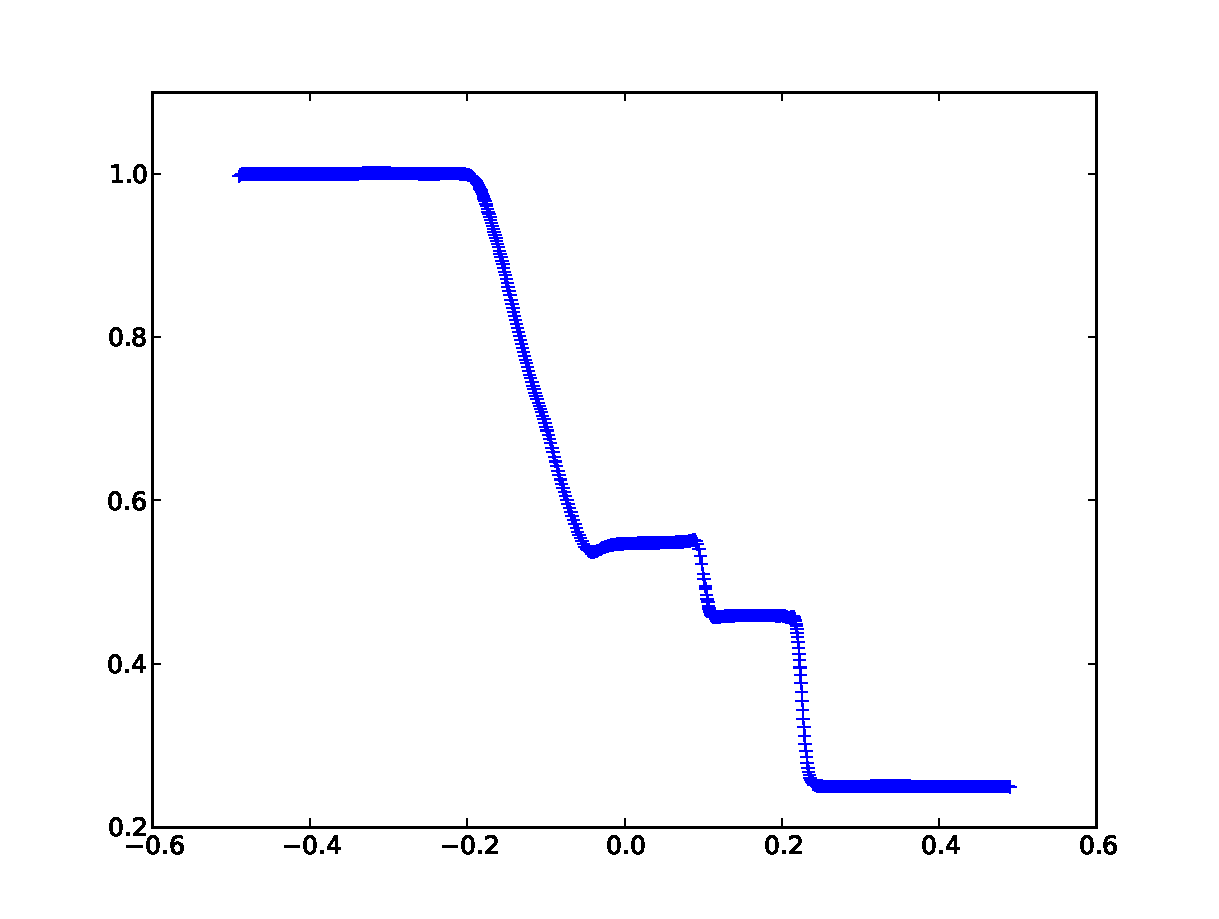
\includegraphics[width=0.5\textwidth]{150.pdf}
\caption{Graph of density with respect to space on the domain 
$[-0.5,0.5]$. At time $t = 0.15$.}
\label{fig:15}
\end{figure}

\begin{figure}[bth]
\centering
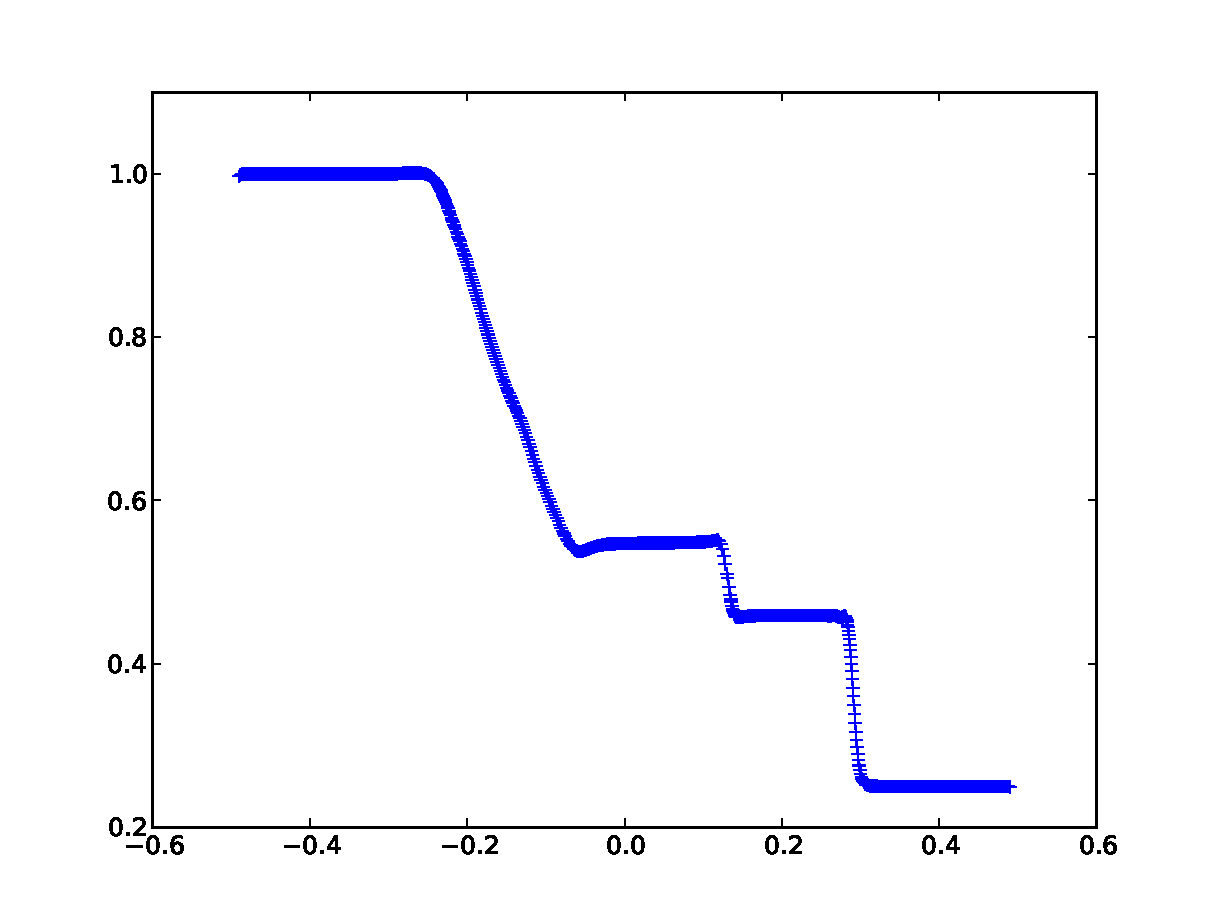
\includegraphics[width=0.5\textwidth]{200.pdf}
\caption{Graph of density with respect to space on the domain 
$[-0.5,0.5]$. At time $t = 0.2$.}
\label{fig:200}
\end{figure}

\subsection{Fortran Comparison} 

We use the fortran code to run an exact Riemann Solver and
 compare the solutions to our SPH code. 

We can see that at small time $t = 0.05$ the two solutions are relatively close
in ~\ref{fig:comp050}. 

\begin{figure}[bth]
\centering
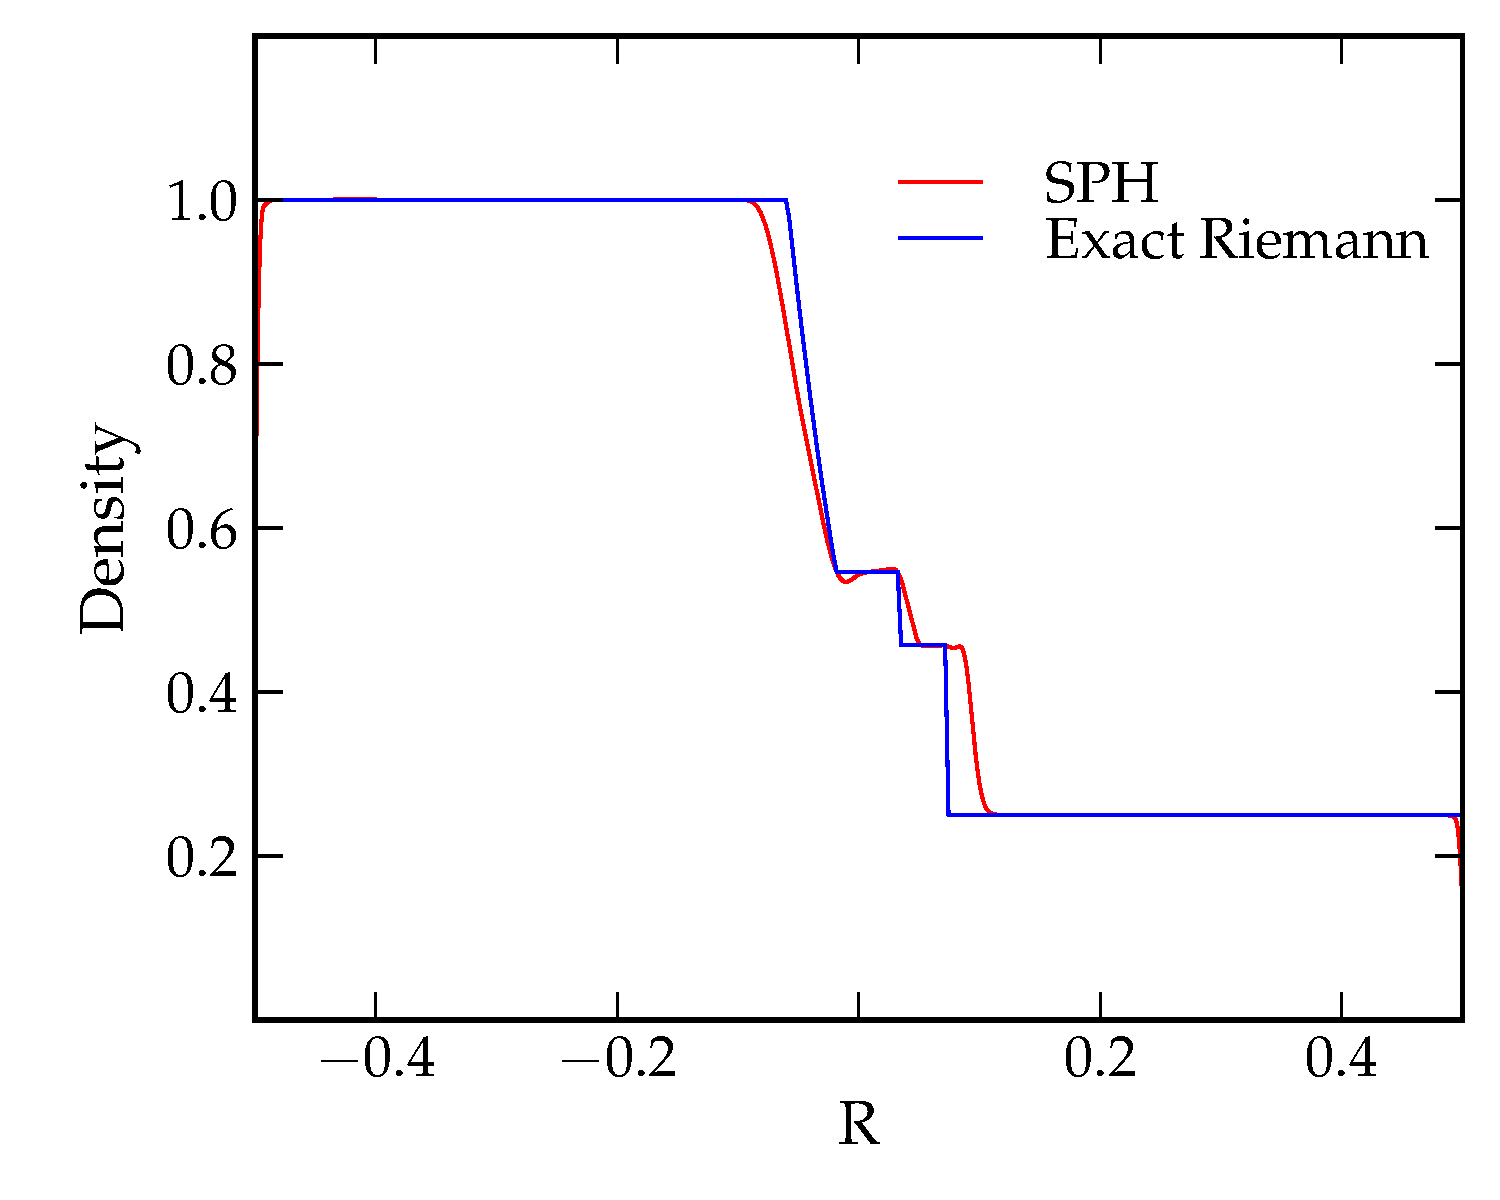
\includegraphics[width=0.5\textwidth]{compare050.pdf}
\caption{Graph of density with respect to space on the domain 
$[-0.5,0.5]$ at $t = 0.05$. SPH solution in red, exact Riemann Solver in blue.}
\label{fig:comp050}
\end{figure}

As time goes on our numerical solution differs from the exact solution, as we 
would expect. At $t=0.105$ the numerical simulation has over done the
rarefraction as well as extended moved the shock to far to the right 
~\ref{fig:comp105}. 


\begin{figure}[bth]
\centering
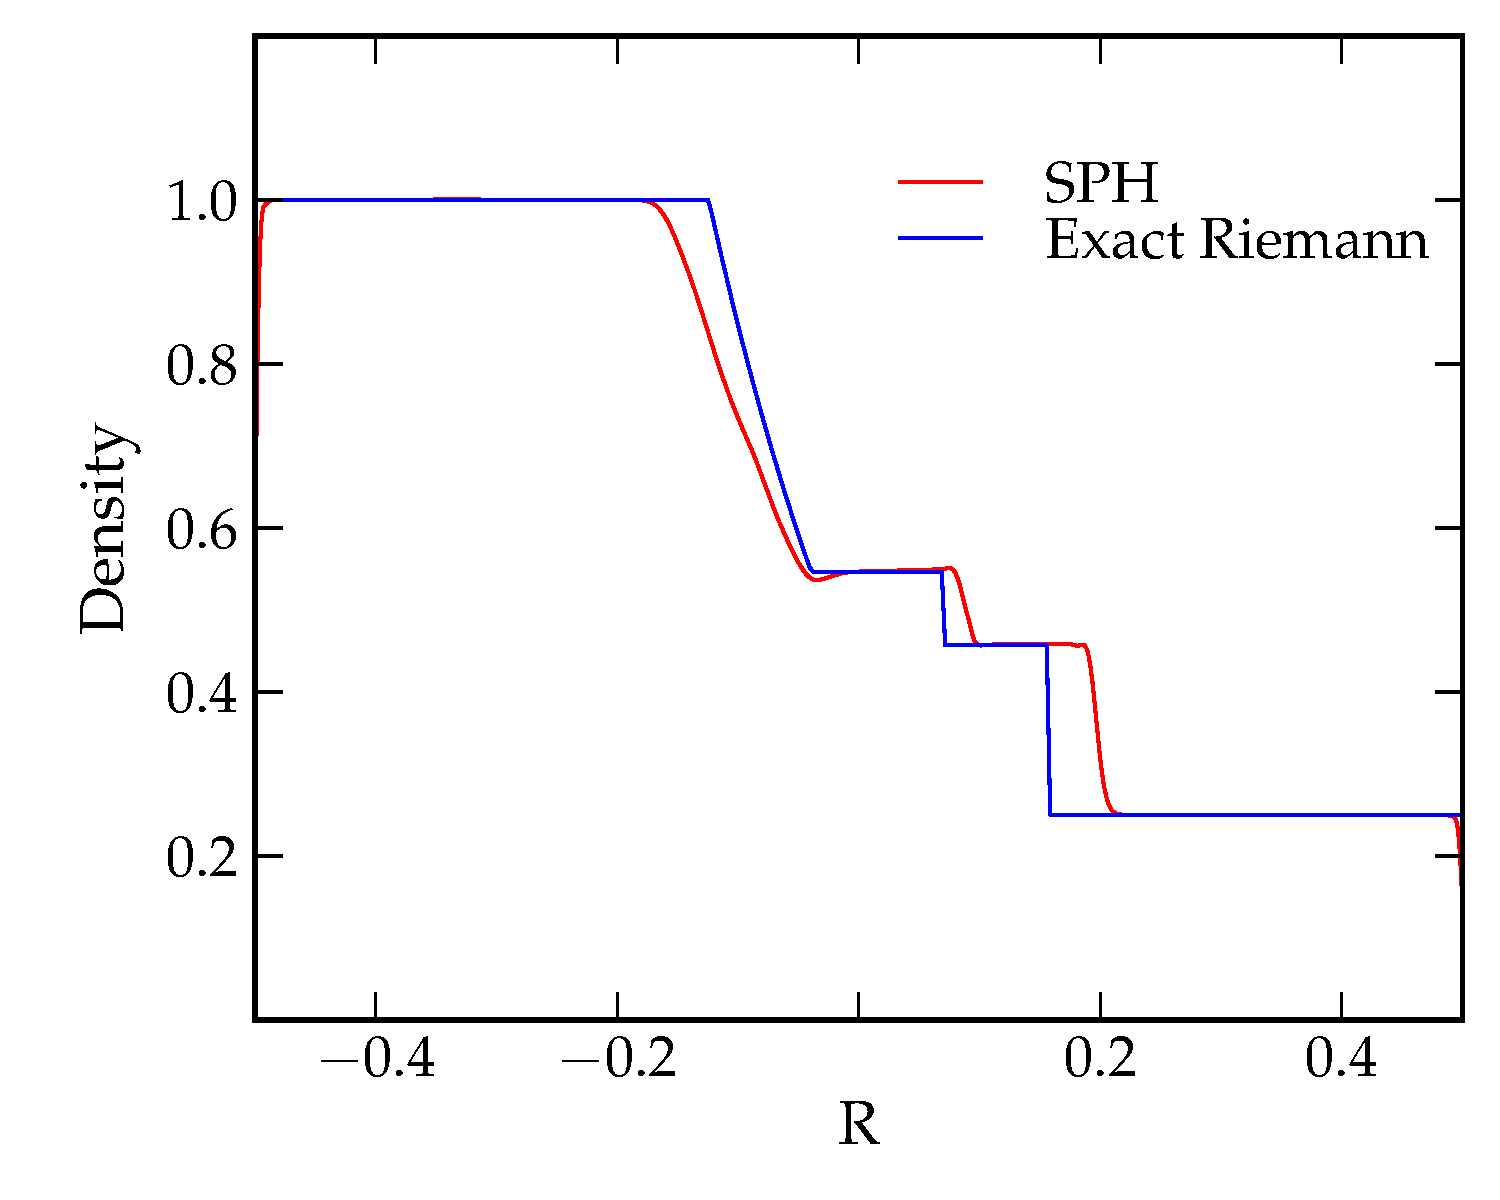
\includegraphics[width=0.5\textwidth]{compare105.pdf}
\caption{Graph of density with respect to space on the domain 
$[-0.5,0.5]$ at $t = 0.105$. SPH solution in red, exact Riemann Solver in blue.}
\label{fig:comp105}
\end{figure}
\end{document}

These problems are only further exacerbated by more time as we can see in 
~\ref{fig:comp150} and ~\ref{fig:comp195}.

\begin{figure}[bth]
\centering
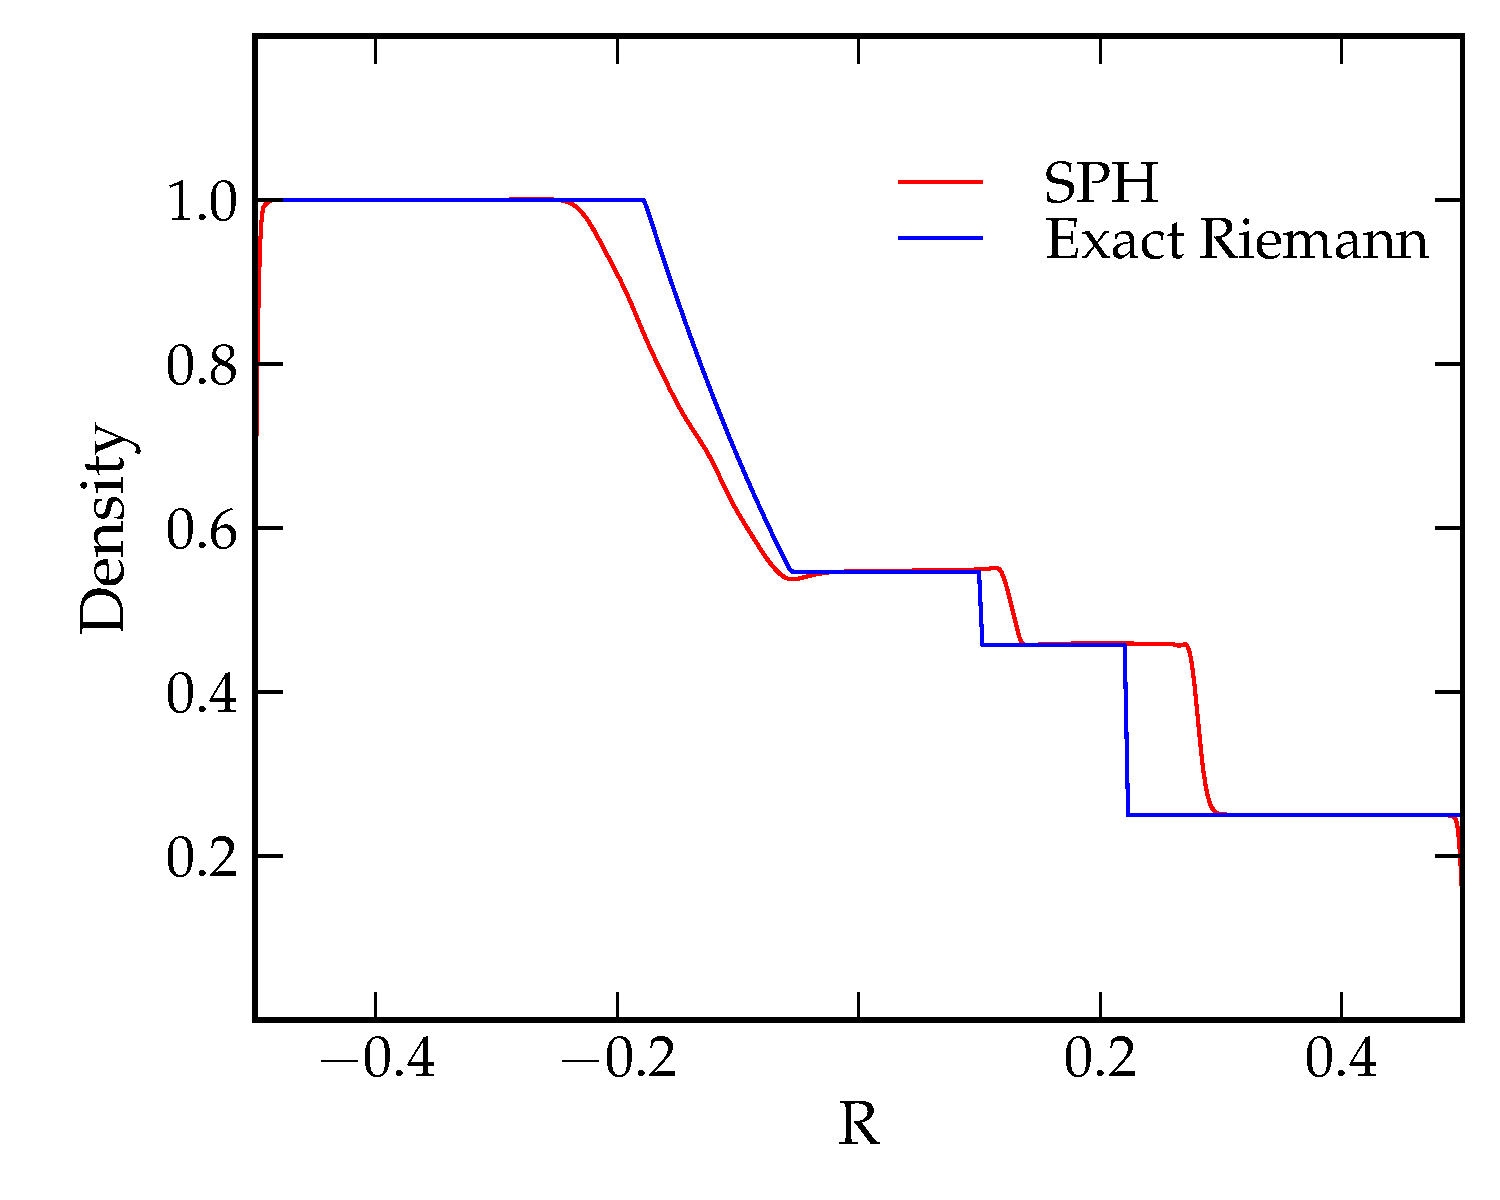
\includegraphics[width=0.5\textwidth]{compare150.pdf}
\caption{Graph of density with respect to space on the domain 
$[-0.5,0.5]$ at $t = 0.150$. SPH solution in red, exact Riemann Solver in blue.}
\label{fig:comp150}
\end{figure}
\end{document}

\begin{figure}[bth]
\centering
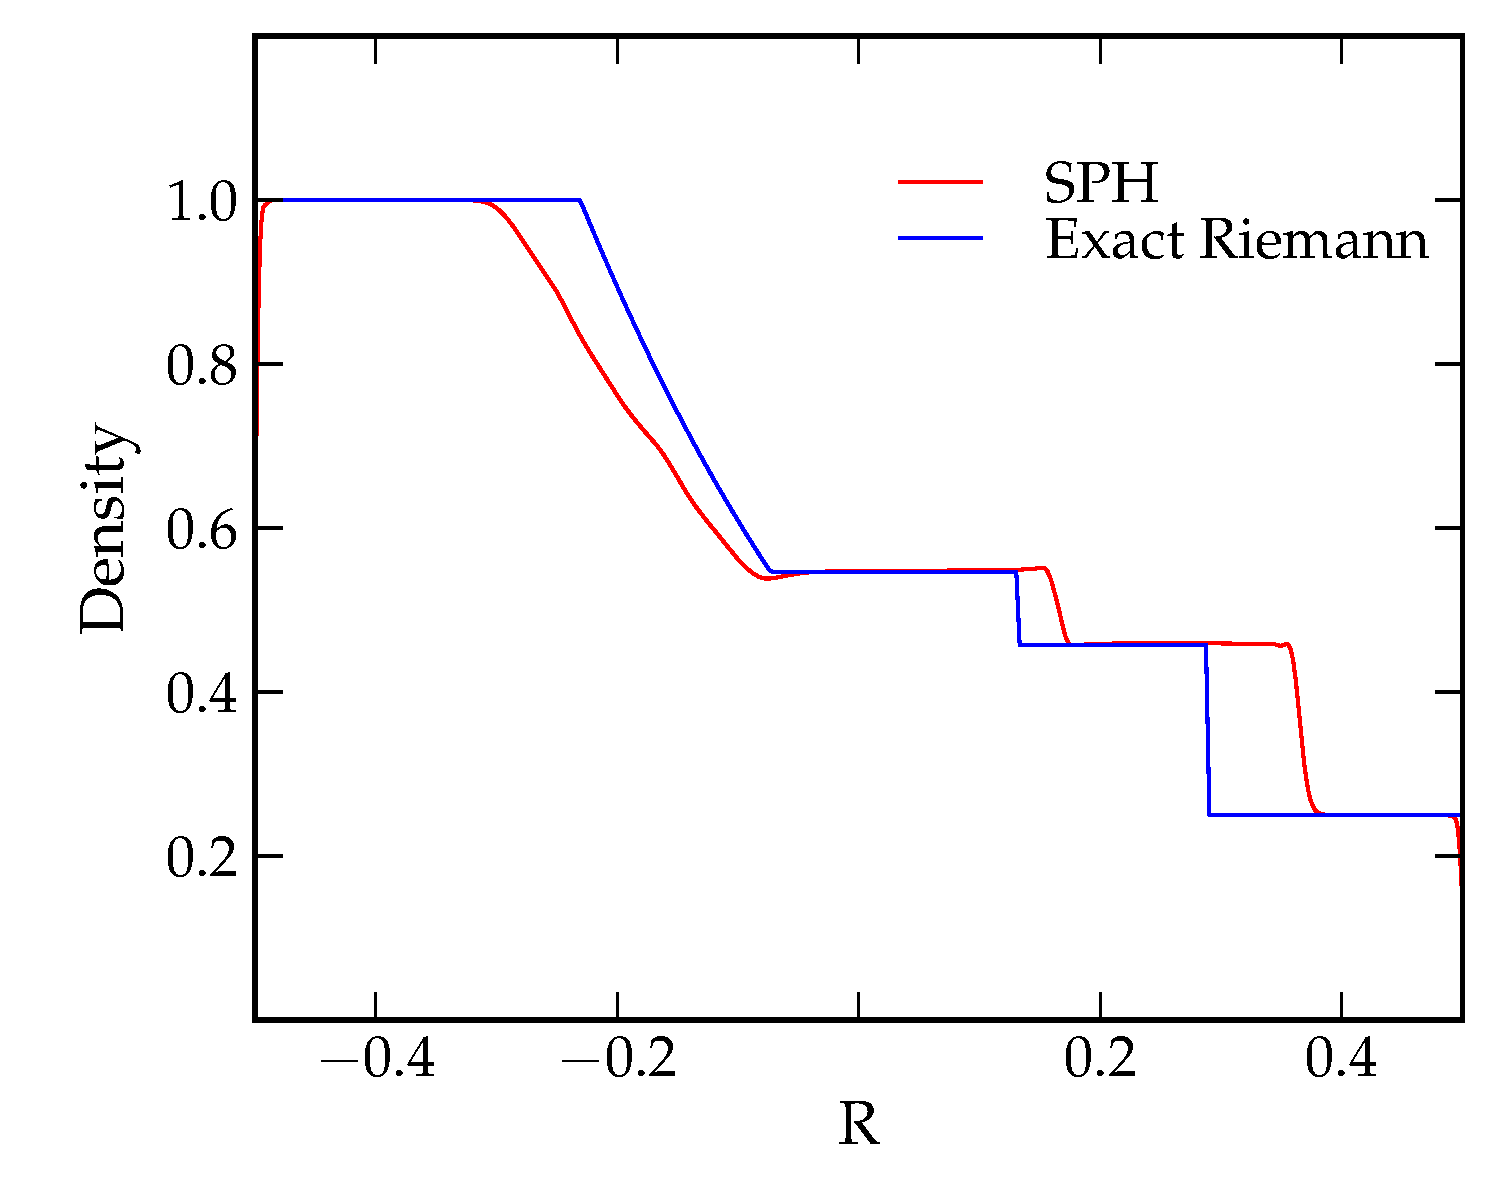
\includegraphics[width=0.5\textwidth]{compare195.pdf}
\caption{Graph of density with respect to space on the domain 
$[-0.5,0.5]$ at $t = 0.195$. SPH solution in red, exact Riemann Solver in blue.}
\label{fig:comp195}
\end{figure}

\end{document}

